\documentclass[11pt,spanish,a4paper]{article}
% Versión 1.er cuat 2021 Víctor Bettachini < bettachini@df.uba.ar >

% Versión 1.er cuat 2021 Víctor Bettachini < bettachini@df.uba.ar >

\usepackage[T1]{fontenc}
\usepackage[utf8]{inputenc}

\usepackage[spanish, es-tabla]{babel}
\def\spanishoptions{argentina} % Was macht dass?
% \usepackage{babelbib}
% \selectbiblanguage{spanish}
% \addto\shorthandsspanish{\spanishdeactivate{~<>}}

\usepackage{graphicx}
\graphicspath{{./figuras/}}
% \usepackage{float}

\usepackage[arrowdel]{physics}
\newcommand{\pvec}[1]{\vec{#1}\mkern2mu\vphantom{#1}}
% \usepackage{units}
\usepackage[separate-uncertainty=true, multi-part-units=single, locale=FR]{siunitx}
\usepackage{isotope} % $\isotope[A][Z]{X}\to\isotope[A-4][Z-2]{Y}+\isotope[4][2]{\alpha}

\usepackage{tasks}
\usepackage[inline]{enumitem}
% \usepackage{enumerate}

\usepackage{hyperref}

% \usepackage{amsmath}
% \usepackage{amstext}
\usepackage{amssymb}

\usepackage{tikz}
\usepackage{tikz-dimline}
\usetikzlibrary{math}
\usetikzlibrary{arrows.meta}
% \usetikzlibrary{snakes}
% \usetikzlibrary{calc}
\usetikzlibrary{decorations.pathmorphing}
\usetikzlibrary{patterns}

\usepackage[hmargin=1cm,vmargin=1.6cm,nohead]{geometry}
% \voffset-3.5cm
% \hoffset-3cm
% \setlength{\textwidth}{17.5cm}
% \setlength{\textheight}{27cm}

\usepackage{lastpage}
\usepackage{fancyhdr}
\pagestyle{fancyplain}
\fancyhead{}
\fancyfoot{{\tiny \textcopyright DF, FCEyN, UBA}}
\fancyfoot[C]{ {\tiny Actualizado al \today} }
\fancyfoot[RO, LE]{Pág. \thepage/\pageref{LastPage}}
\renewcommand{\headrulewidth}{0pt}
\renewcommand{\footrulewidth}{0pt}


\begin{document}
\begin{center}
	\textbf{Física 2} (Físicos) \hfill \textcopyright {\tt DF, FCEyN, UBA}\\
	\textsc{\LARGE Interferencia por división de frente de onda}
\end{center}

Los ejercicios con (*) entrañan una dificultad adicional. Son para investigar después de resolver los demás.


\begin{enumerate}

\subsection*{Interferómetro de Young}

\item En el experimento de Young.
\begin{enumerate}
	\item ¿Cuál es el lugar geométrico de los puntos que reciben ondas con la misma diferencia de fases?
	\item Si la pantalla de observación está lo suficientemente alejada de las ranuras, ¿qué aspecto tienen las franjas de interferencia?
\end{enumerate}


\item 
\begin{minipage}[t][2.4cm]{0.6\textwidth}
Una fuente monocromática de $\lambda = \SI{5500}{\angstrom}$ ilumina un dispositivo de Young.
La distancia entre ranuras es $s = \SI{3.3}{\milli\metre}$, y de estas a una pantalla $D = \SI{3}{\metre}$.
Calcule la interfranja $i$.
\end{minipage}
\begin{minipage}[c][4cm][t]{0.35\textwidth}
	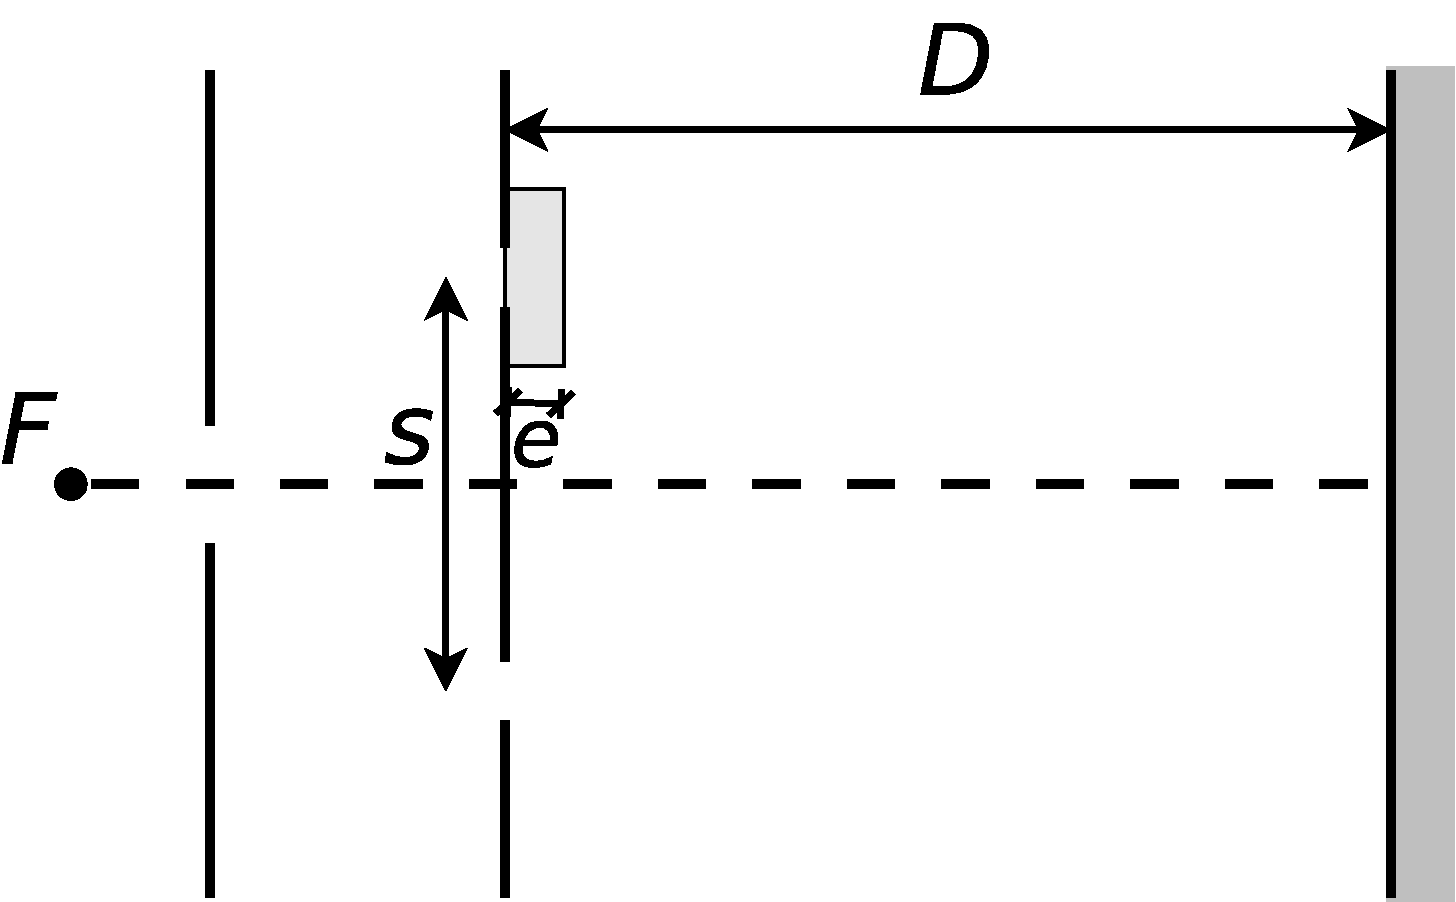
\includegraphics[width=\textwidth]{ej5-5}
\end{minipage}
Si se coloca detrás de una de las ranuras una lámina de vidrio de caras planas paralelas de un espesor $e = \SI{0.01}{\milli\metre}$ como muestra la figura, el patrón de franjas se deplazará.
Determine el sentido de tal desplazamiento y la fórmula que da la expresión de dicho desplazamiento.
Sabiendo que las franjas se han desplazado \SI{4.73}{\milli\metre}, calcule el valor del índice de refracción del vidrio.
¿Puede detectar dicho corrimiento con una fuente monocromática?
¿Y con una policromática?


\item ¿Cómo cambia el experimento de Young si la fuente luminosa no está simétricamente situada respecto de la ranura, o si, por algún motivo, las ondas que llegan a las mismas tienen un cierto desfasaje?
¿Cómo puede detectar dicho corrimiento?



%\item
%\begin{minipage}[t][5cm]{0.6\textwidth}
%(*) Se tiene el dispositivo para producir interferencia que indica la figura.
%La fuente puntual monocromática de longitud de onda $\lambda$ (linealmente polarizada en el eje $z$, con amplitud $E_{0}$), ilumina dos rendijas separadas por una distancia $a$.
%La fuente está centrada respecto de las rendijas y se encuentra a una distancia $L_{0}$ de las mismas.
%A la izquierda de las rendijas hay dos medios distintos; sobre el eje $x$ es $n_{1}$, y debajo del eje $x$ es $n_{2}$ ($n_{2}>n_{1}$); a la derecha de las rendijas el índice es $n_{1}$ solamente.
%A continuación de la rendija 2 se coloca una lámina polarizadora cuyo eje de transmisión forma un ángulo $\alpha$ con el eje $z$. 
%Datos: $a$, $n_{2}$, $n_{1}$, $E_{0}$, $L_{0}$, $L$.
%\end{minipage}
%\begin{minipage}[c][0cm][t]{0.35\textwidth}
%	\includegraphics[width=\textwidth]{ej5-7}
%\end{minipage}
%\begin{enumerate}
%	\item ¿Qué efecto produce en el patrón de interferencia la diferencia de medios?
%	Explique.
%	\item Halle el campo eléctrico que sale de la lámina polarizadora como función de $\alpha$; expréselo en las coordenadas $y-z$ (sólo el campo que sale de la ranura 2; no el total).
%	\item Halle la expresión de la intensidad en un punto $P$ de la pantalla, en función de los campos eléctricos a la salida de las rendijas 1 y 2.
%	Tenga en cuenta para esto la polarización de dichos campos.
%	\item Calcule el contraste $c=\frac{I_{m\acute{a}x}-I_{m\acute{\imath}n}}{I_{m\acute{a}x}\text{+}I_{m\acute{\imath}n}}$, en función del ángulo $\alpha$ y de $\theta$ (ángulo subtendido por P).
%	¿Existen ceros de intensidad para algún $\theta$?
%\end{enumerate}

\subsection*{Espejos de Fresnel}

\item 
\begin{minipage}[t][4.2cm]{0.6\textwidth}
Se usa como fuente luminosa para un par de espejos de Fresnel una ranura $D$ iluminada con luz monocromática de \SI{4000}{\angstrom} y colocada a \SI{20}{\centi\metre} de la intersección de los espejos sobre la bisectriz.
Las franjas de interferencia observadas a \SI{1}{\metre}  de distancia del vértice de los espejos tienen una interfranja de \SI{1}{\milli\metre}.
Calcular el ángulo $\alpha$ entre los planos de los espejos.
La distancia vértice-pantalla: \SI{1}{\metre} y $d = \SI{20}{\centi\metre}$.
Note que la fuente y las dos imágenes son equidistantes de la intersección de los espejos. 
\end{minipage}
\begin{minipage}[c][0cm][t]{0.35\textwidth}
	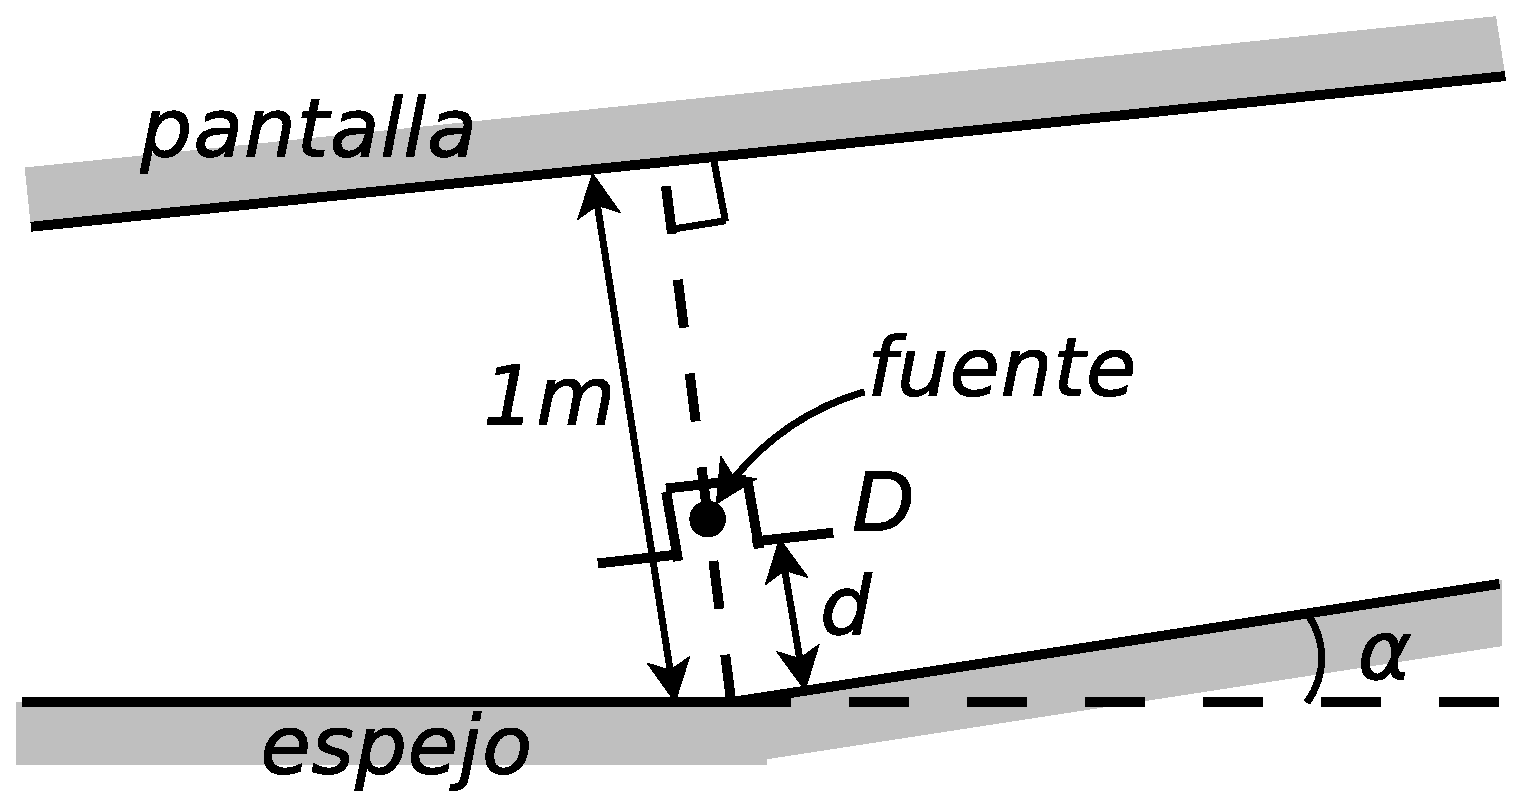
\includegraphics[width=\textwidth]{ej5-8}
\end{minipage}



\item En un experimento de interferencia con espejos de Fresnel, ¿qué parámetros deben modificarse para que la interfranja disminuya?



\item (*) Examinadas con una lupa de distancia focal $f = \SI{5}{\centi\metre}$, dos franjas de interferencia consecutivas, producidas con los espejos de Fresnel, se encuentran a una separación aparente $i' = \SI{3}{\milli\metre}$.
	La distancia entre las imágenes de la fuente y la pantalla es $D = \SI{4}{\metre}$ y la separación entre las dos imágenes es $d = \SI{4}{\milli\metre}$.
	¿En qué longitud de onda emite la fuente?
	Nota: suponer que la imagen de las franjas se forma a una distancia $D_v = \SI{25}{\centi\metre}$ (distancia de visión clara) de la lupa.





\subsection*{Espejos de Lloyd}

\item (*) ¿Por qué motivo se puede concluir, en el experimento del espejos de Lloyd, que la luz reflejada ha sufrido un desfasaje de \ang{180;;}?

\subsection*{Biprisma de Fresnel}

\item 
\begin{minipage}[t][2.7cm]{0.6\textwidth}
\begin{enumerate}
	\item Analice cómo se producen las imágenes virtuales en un biprisma de Fresnel.
	\item ¿Qué ocurre con la posición de las imágenes si se da vuelta el biprisma, es decir, si la arista enfrenta a la pantalla en vez de enfrentar a la fuente?
\end{enumerate}
\end{minipage}
\begin{minipage}[c][1.5cm][t]{0.35\textwidth}
	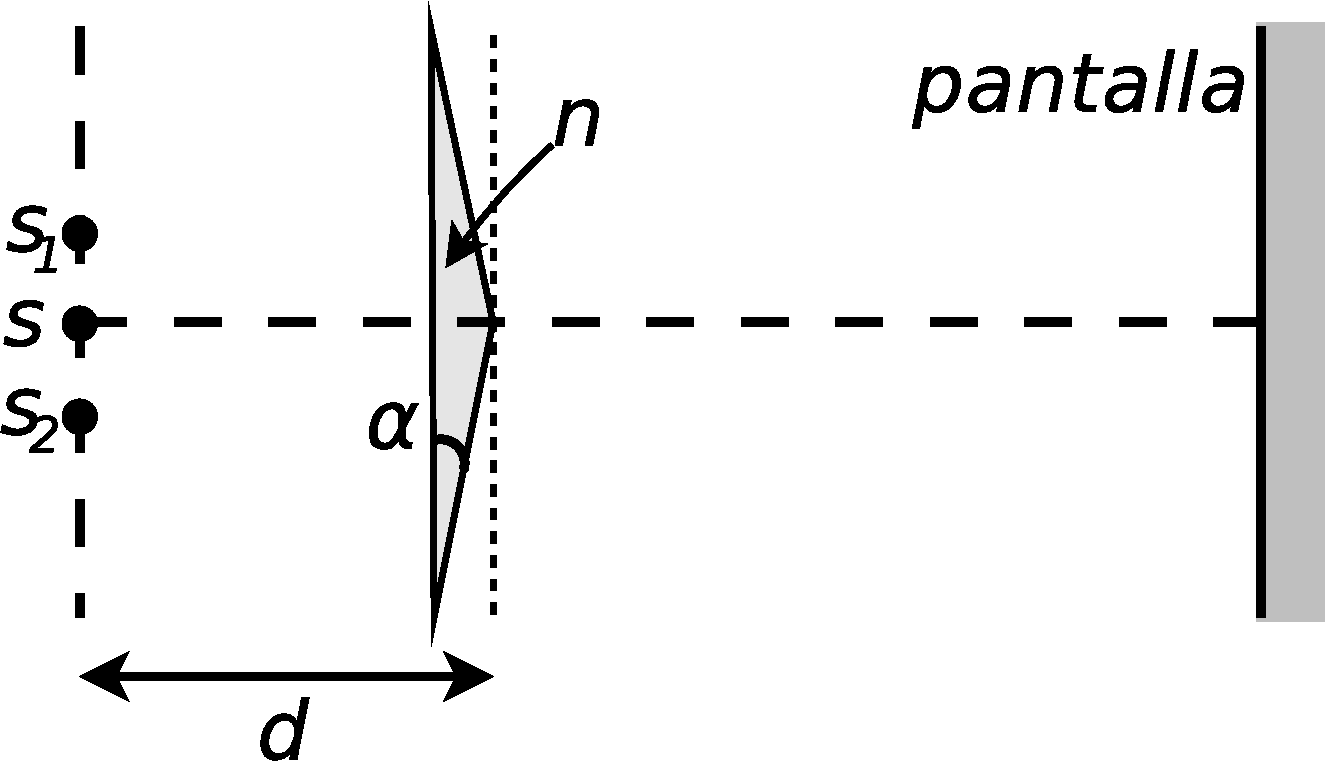
\includegraphics[width=\textwidth]{ej5-11}
\end{minipage}



\item Con vídrio Crown se construyó un biprisma de Fresnel con ángulo de \ang{1;;}.
Se ubica una pantalla a \SI{60}{\centi\metre} del biprisma y una fuente luminosa a \SI{15}{\centi\metre} de éste.
Calcular el ancho de las interfranjas observadas con luz roja (línea C de Fraunhofer) y luz azul (línea F de Fraunhofer).
Extraer las longitudes de onda y los índices de refracción de tablas.



\item Se observan franjas de interferencia con un biprisma de Fresnel con ángulo de \ang{1.5;;} e índice de refracción \num{1.5}.
Para esto se usa una fuente de luz de \SI{4000}{\angstrom} situada a \SI{5}{\centi\metre} del vértice, y una pantalla situada a \SI{1}{\metre} del biprisma.
Si, dejando todas las demás condiciones iguales, se cambia el biprisma por uno de ángulo \ang{3;;} e índice \num{1.6}; ¿en cuánto varió la interfranja?


\item En un experimento de interferencia con un biprisma de Fresnel, ¿qué parámetros se pueden modificar para que la interfranja aumente?


\item 
\begin{minipage}[t][3cm]{0.6\textwidth}
(*) Se tiene un dispositivo para producir interferencia consistente en una fuente puntual y monocromática $S$, que emite con longitud de onda $\lambda$, que se encuentra a una distancia $D_1$ de un biprisma compuesto por dos prismas delgados de distintos índices y ángulos: $n_1$, $\alpha_1$ ($y>0$) y $n_2$, $\alpha_2$ ($y<0$).
El dispositivo se muestra en la figura.
\end{minipage}
\begin{minipage}[c][2cm][t]{0.35\textwidth}
	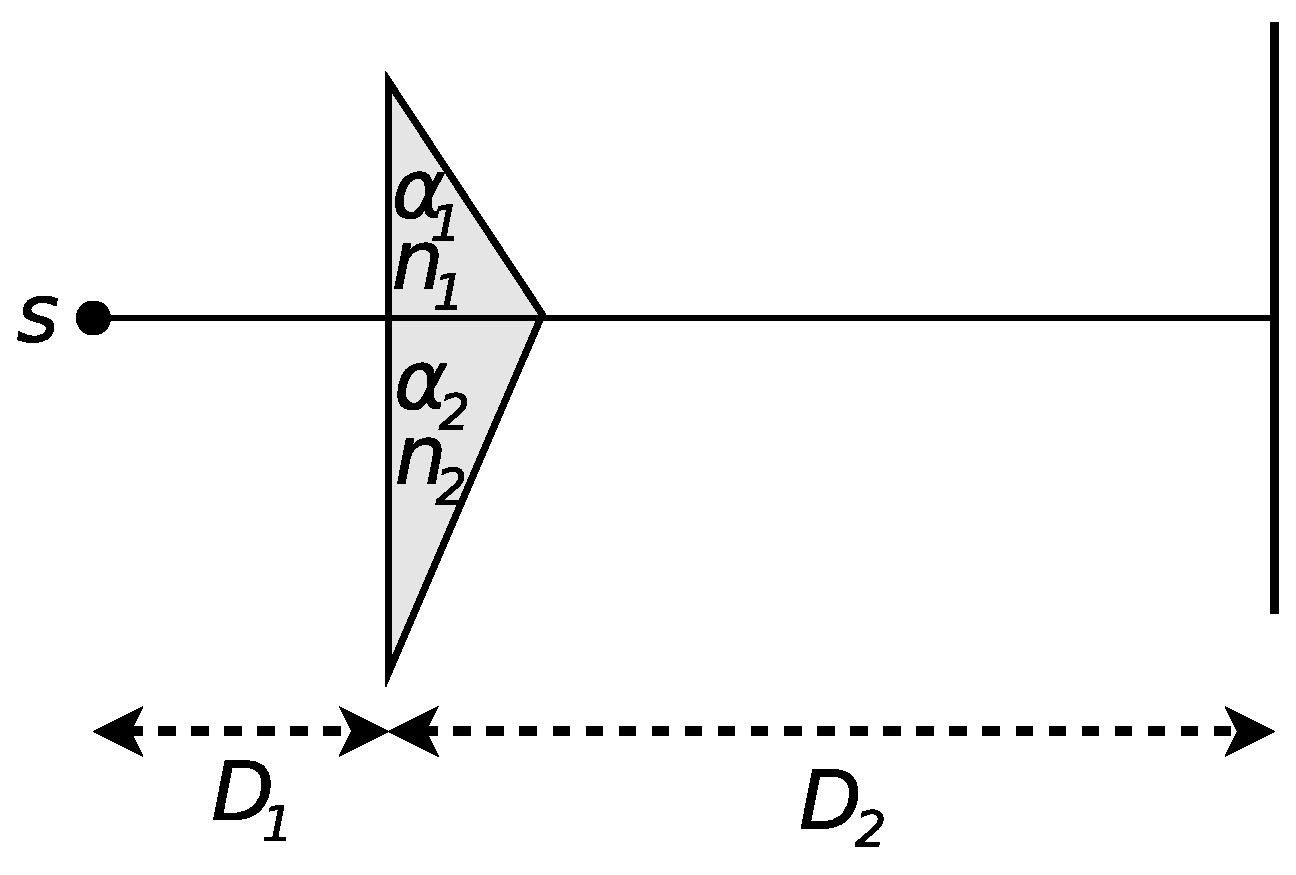
\includegraphics[width=\textwidth]{ej5-15}
\end{minipage}
\begin{enumerate}
	\item Hallar la ubicación de las imágenes $S_1$ y $S_2$ por la refracción en ambas zonas del biprisma, que observaría una persona ubicada a la derecha del mismo. 
	\item Marque en una figura la zona donde se produce la interferencia.
	\item Para un punto $P$ genérico sobre la pantalla, calcule el desfasaje $\delta$. Sugerencia: piense en los rayos que llegan a $P$ como provenientes de las imágenes halladas en a).
	\item Calcule la interfranja sobre la pantalla. 
	\item Halle la posición de los máximos sobre la pantalla.
	Si Ud. observara este fenómeno sin conocer los parámetros del dispositivo, ¿qué podría hacer para distinguir cuál es el orden con $m = 0$? 
	\item ¿Cómo debe ser la relación $\alpha_1/\alpha_2$ para que el máximo con $m = 0$ esté en la línea determinada por la fuente y el vértice del biprisma?
\end{enumerate}



\section*{Resumen: interferómetros por división de frente de onda}
\item Diga qué entiende por interferómetro por división de frente de onda.
Mencione los más representativos, haga un esquema de cada uno de ellos e indique sus parámetros característicos.


\end{enumerate}

\end{document}
